\documentclass{beamer}
\usepackage[utf8]{inputenc}
\usepackage[portuguese]{babel}
\usepackage{amsmath}
\usepackage{subfigure}
\usepackage{booktabs}
\usepackage{mhchem}             % chemical reactions
\usetheme{metropolis}           % Use metropolis theme

\newtheorem{mydefinition}{Definição}

\newcommand{\foreignword}[1]{\textit{#1}}
\newcommand{\toolname}[1]{\textit{#1}}
\newcommand{\fieldR}{\mathbb{R}}
\newcommand{\powerset}{\mathcal{P}}
\newcommand{\probability}{\mathbb{P}}
\newcommand{\expectation}{\mathbb{E}}
\newcommand{\algname}[1]{\texttt{#1}}
\newcommand{\langname}[1]{\texttt{#1}}
\newcommand{\varname}[1]{\texttt{#1}}
\newcommand{\floor}[1]{\lfloor #1 \rfloor}
\newcommand{\ceil}[1]{\lceil #1 \rceil}
\newcommand{\mathsc}[1]{{\normalfont\textsc{#1}}}
\newcommand{\species}[1]{\textit{#1}}
\newcommand{\gender}[1]{\textit{#1}}

\graphicspath{ {img/} }

\title{Identification of cell signaling pathways based on biochemical 
reaction kinetics repositories}
\date{May 2019}
\author{Gustavo Estrela}
\institute{Instituto de Matemática e Estatística \\ 
           Centro de Toxinas, Resposta-imune e Sinalização Celular (CeTICS) \\
           Laboratório Especial de Ciclo Celular, Instituto Butantan}
\begin{document}
\maketitle
    
%Introduction
%- Cell Signaling Pathways;
%- Modeling it mathematically;
%- With a computational working computational model, we can enlight the
%  structure of a change of behaviour of a cell;
%- Creating a model;
    %- find a set of reactions;
    %- estimate the parameters of this model;
%- Lulu Wu created a method that systematically searches for a model, 
  %modifying it incrementally
    %- we can see the problem as a feature selection problem;
    %- it didn't work out so well...
    %- she was only able to reconstruct models if the starting model was
      %already similar to the correct model
    %- this may have happened because: the database could be more nearly
      %complete; the search algorithm could be more general; her cost 
      %function could not penalize well overcomplex functions.
%- We propose then to create a new methodology that overcomes theses 
  %difficulties using a new cost function, defining a broader search 
  %space and using new search algorithms.
%- Objectives of this work.



\section{Introduction}
\begin{frame}{Cell Signaling}
% Antes de mais nada, vamos entender o que são vias de sinalização 
% celular. 
% A sinalização celular faz parte da comunicação das células de um 
% organismo. Um sinal pode avançar 

%\begin{itemize}
%\item{
Cell signaling pathways are important structures that allow cells
to respond to signals that come from its environment.
%}
\pause
%\item{

This mechanism is essential for many cell functions, including 
reproduction, growth and death.
%}
\pause
%\item{

Understanding the functioning of cell signaling is important in many 
biological areas.
%}
%\end{itemize}
\end{frame}


\begin{frame}{Cell Signaling}
\begin{figure}
    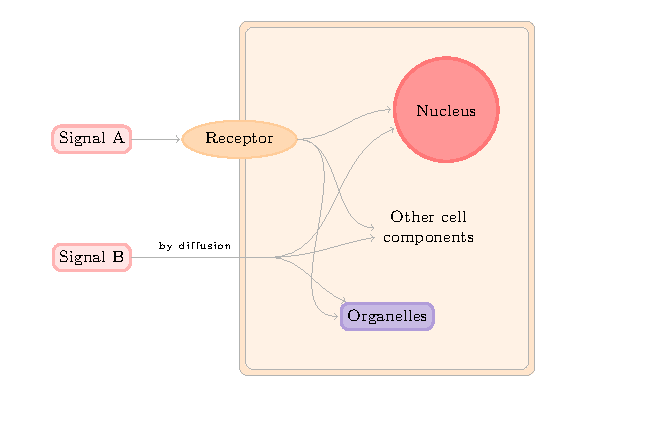
\includegraphics[clip=True, scale=.85]{introduction/signaling_mechanism.pdf}
    \caption{A general cell signaling mechanism.}
\end{figure}
\end{frame}

\begin{frame}{Cell Signaling Pathways}
A cell signaling network can be characterized by a sequence of chemical 
reactions that allows the presence of a signal to modify the state or 
behaviour of a cell.
\begin{figure}
    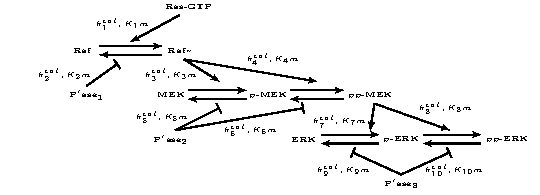
\includegraphics{introduction/csp_example.pdf}
    \caption{An example of a signaling pathway.}
\end{figure}
\end{frame}

\begin{frame}{Mathematical Models of Signaling Networks}
In many applications, we summarize the state of the cell with a 
measurement based on the concentration of chemical species of the cell.
\pause

Using biochemical and enzymatic kinetics, we can write equations that
represent the rate of change of concentration for a chemical species.
\end{frame}


\begin{frame}{Mathematical Models of Signaling Networks}
As an example, for the chemical reaction
\begin{equation*}
\ce{
    A -> B
},
\end{equation*}

\pause
we can write the following equation:
\begin{equation*}
        \frac{d[\text{A}]}{dt} = k_1[\text{A}]; 
\end{equation*}
where $k_1$ is a reaction rate constant.

\pause
Repeating this procedure for all reactions of a pathway allows us to 
derive a system of ordinary differential equations that can model the 
signaling pathway.
\end{frame}


\begin{frame}{Identification of Cell Signaling Pathways}
The problem of identification of cell signaling pathways is the problem
of finding the components of a signaling pathway and how they interact
given a set of experimental measurement.

\pause
As the input, a description of a biological experiment and a set of 
experimental measurements are given. A possible output to the problem is
a mathematical model of the pathway, \pause composed by:
\begin{itemize}
    \item{a set of chemical reactions that are relevant for the 
        biological experiment;}
    \pause
    \item{information about the reaction rate constants of the model.}
\end{itemize}
\end{frame}


\begin{frame}{Identification of Cell Signaling Pathways}
One can search for the set of chemical reactions relevant for a 
biological experiment in repositories like the Kyoto Encyclopedia of 
Genes and Genomes (KEGG). \pause However, the pathway maps from KEGG may
be incomplete or have impertinent reactions for the biological 
experiment of interest.
\pause

Hence, it is desirable to construct a method that can systematically 
modify these models and choose the one that better represents the 
experiment.
\end{frame}


\begin{frame}{Identification of Cell Signaling Pathways}
Lulu Wu (2015) presented in her master dissertation a methodology that 
proposes to systematically modify models of signaling network in order
to better represent experiments.
\pause

On her work, the problem of identification of cell signaling pathways is
treated as a feature selection problem.
\end{frame}


\begin{frame}{Feature Selection Problem}
The feature selection problem is a combinatorial optimization problem:
\begin{center}
Given a set of features $S$ and a cost function $c$, find subset 
        $X \in \powerset (S)$, with minimum cost $c(X)$.
\end{center}

\pause
\begin{figure}
    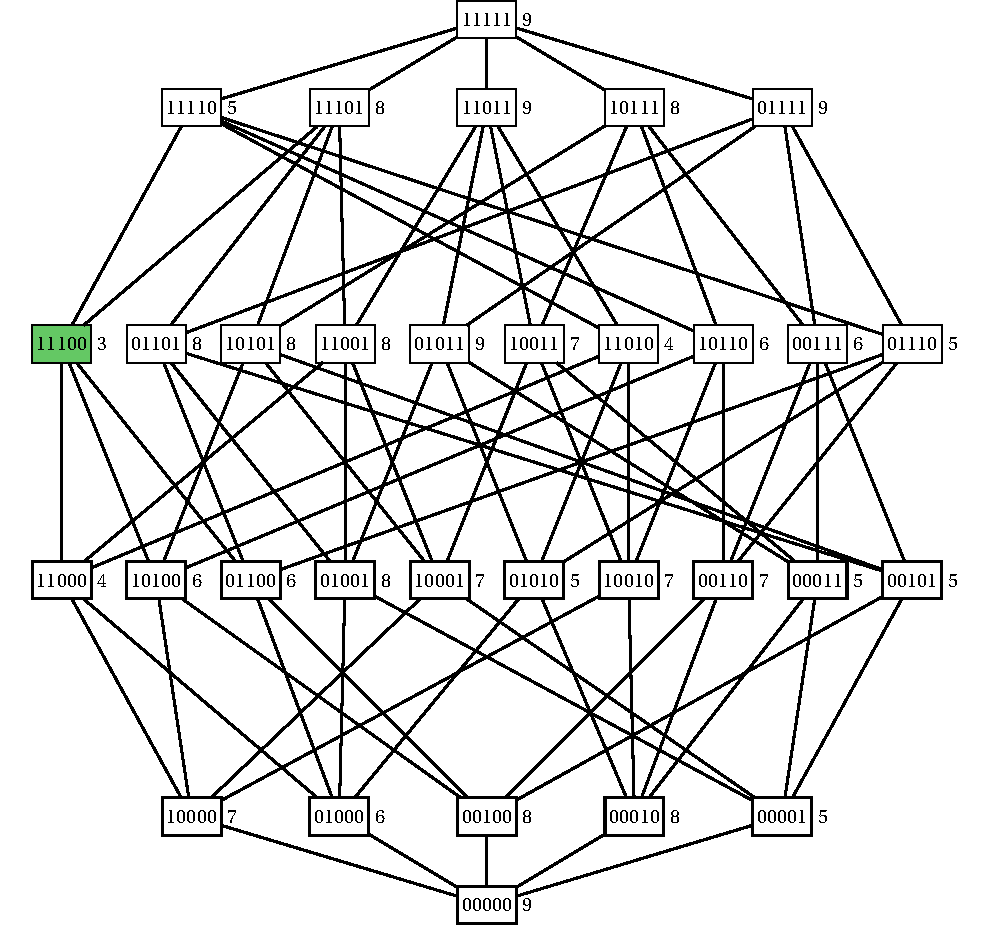
\includegraphics[scale=.24]{introduction/Boolean_lattice.pdf}
    \caption{An example of feature selection search space with 5 
    features.}
\end{figure}
\end{frame}


\begin{frame}{Feature Selection for Identification of Signaling Pathways}
If we consider that the set of all possible chemical reactions is the
set of features, than we can tackle the identification of signaling 
pathway problem as a feature selection problem.
\end{frame}

%\begin{frame}{Mathematical Models of Signaling Pathways}
%To build a model of a signaling pathway we must accomplish two tasks:
%\begin{itemize}
    %\pause
    %\item{Determine a set of chemical reactions that is relevant in
        %the pathway.}
    %\pause
    %\item{Determine values for the reactions rate constants.}
%\end{itemize}
%Theses tasks can be accomplished by looking for static interactome maps
%in directories 
%\end{frame}


%Fundamental Concepts
%- How are the experimental measures taken
    %- A few details about the procedure
%- How can we model cell signaling pathways mathematically
    %- kinetics laws
    %- M.M. simplifcations
%- How can we choose between models
    %- Approximate Bayesian Computation
    %- Annealing-Melting Integration
\section{Fundamental Concepts}

%Model Selection
%- Approximate Bayesian Computation
    %- What does it do;
    %- ABC-SMC algorithm
%- A method using Thermodynamic Integration
    %- What does it do;
    %- How to derive the thermodynamic integration
    %- How to estimate this value
% Implementations
\section{Model Selection}


\section{Experiments on Model Selection}
\begin{frame}
\end{frame}
\section{Next Steps}

\end{document}


